% =============================================================================
% Artigo científico (template SBC) derivado da monografia em ../article/.
% Compilação (pdflatex):
%   pdflatex main && bibtex main && pdflatex main && pdflatex main
% Tabelas e figuras de resultados são reutilizadas de ../article/ (geradas por
% ../article/scripts/gerar_resultados.py a partir de data/outputs/*.parquet).
% =============================================================================
\documentclass[12pt]{article}

\usepackage{sbc-template}
\usepackage[T1]{fontenc}
\usepackage[utf8]{inputenc}
\usepackage[brazilian]{babel}
\usepackage{graphicx,url}
\usepackage{booktabs}
\usepackage{array}
\usepackage{amsmath,amssymb}
\usepackage{tikz}
\usetikzlibrary{positioning, arrows.meta, fit, backgrounds, shapes.geometric}
% hyperref omitido: com o sbc-template.sty, gera erro "Undefined control
% sequence \normalsfcodes" no TeX Live 2026.

% Sinal de menos (U+2212) usado nas tabelas geradas.
\DeclareUnicodeCharacter{2212}{\ensuremath{-}}

% Equivalentes dos comandos \fonte e \nota do abnTeX2, usados pelas tabelas
% geradas em ../article/tabelas/: texto pequeno, justificado, abaixo do float.
\newcommand{\fonte}[1]{\par\vspace{3pt}{\footnotesize\leftskip=0.8cm\rightskip=0.8cm
  \parfillskip=0pt plus 1fil\parindent=0pt Fonte: #1\par}}
\newcommand{\nota}[1]{\par\vspace{1pt}{\footnotesize\leftskip=0.8cm\rightskip=0.8cm
  \parfillskip=0pt plus 1fil\parindent=0pt Nota: #1\par}}

% Autoria das fontes das tabelas geradas (../article/scripts/gerar_resultados.py)
\newcommand{\elaboradopor}{Elaborado pelos autores}

\setlength{\emergencystretch}{2em}

% Posicionamento de floats: permite tabelas grandes no topo de páginas com texto.
\renewcommand{\topfraction}{0.9}
\renewcommand{\bottomfraction}{0.8}
\renewcommand{\textfraction}{0.1}
\renewcommand{\floatpagefraction}{0.8}
\setcounter{topnumber}{3}
\setcounter{totalnumber}{4}
\sloppy

\title{Desenvolvimento de uma Ferramenta de Software para Auditoria Algorítmica e Detecção de Vieses em Modelos Preditivos do ENEM}

\author{Roberto Otávio Pereira Leite\inst{1}, Roberta Macêdo Marques Gouveia\inst{1}}

\address{Departamento de Estatística e Informática\\
  Universidade Federal Rural de Pernambuco (UFRPE) -- Recife, PE -- Brasil
  \email{\{roberto.opleite, roberta.gouveia\}@ufrpe.br}
}

\begin{document}

% Faixa institucional (UFRPE à esquerda, BSI à direita) acima do título;
% logos reutilizados da capa da monografia, sem numeração nem legenda.
% A faixa é desenhada só na página 1, por cima da página já montada (gancho
% shipout/foreground do núcleo do LaTeX; origem no canto superior esquerdo),
% na margem superior: não entra no fluxo vertical, de modo que título,
% resumos e quebras de página ficam idênticos aos da versão sem logos.
\newlength{\logoesq}
\setlength{\logoesq}{\dimexpr 1in+\hoffset+\oddsidemargin\relax}
\AddToHookNext{shipout/foreground}{%
  \put(\logoesq,-3.1cm){\hbox to \textwidth{%
    
\includegraphics[height=1.5cm,keepaspectratio]{../article/figuras/logo_ufrpe_horizontal.png}%
    \hfill
    
\includegraphics[height=1.5cm,keepaspectratio]{../article/figuras/logo_bsi.pdf}}}}

\maketitle

\begin{abstract}
Models trained on educational data may amplify inequalities that conventional metrics miss. This paper presents AuditEdu-XAI, a Design Science Research artifact, with a free public interface, that audits, on the test set only, XGBoost classifiers of three ENEM editions with Disparate Impact, group error rates and TreeSHAP. All non-white groups and incomes up to 2.5 minimum wages violate the four-fifths rule in all three editions, and the model amplifies the race/color disparity in the labels in 14 of 15 group-edition combinations (13 with a 95\% CI entirely below zero). Flipping 50\% of the positive training labels of \textit{pardo} candidates, with a negative control, brought the group's Disparate Impact to near zero; the ROC AUC changed, on average, by at most 0.032.
\end{abstract}

\begin{resumo}
Modelos treinados com dados educacionais podem amplificar desigualdades invisíveis às métricas usuais. Apresenta-se o AuditEdu-XAI, artefato de \textit{Design Science Research}, com interface pública e gratuita, que audita, só no conjunto de teste, classificadores XGBoost de três edições do ENEM com Impacto Disparate, taxas de erro por grupo e TreeSHAP. Todos os grupos não brancos e rendas de até 2,5 salários mínimos violam a regra dos quatro quintos nas três edições, e o modelo amplifica a disparidade de raça/cor dos rótulos em 14 de 15 combinações grupo-edição (13 com IC95\% inteiramente negativo). Rebaixar 50\% dos rótulos positivos de treino dos pardos, com controle negativo, quase zerou seu Impacto Disparate; a AUC-ROC variou, em média, até 0,032.
\end{resumo}


\section{Introdução}
\label{sec:introducao}

Impulsionada pela Mineração de Dados Educacionais (MDE), a tomada de decisão orientada a dados vem sendo adotada na gestão educacional para alocar recursos, prever a evasão e estimar o desempenho acadêmico de estudantes \cite{romero2010educational}. No Brasil, os microdados do Exame Nacional do Ensino Médio (ENEM), publicados pelo Instituto Nacional de Estudos e Pesquisas Educacionais Anísio Teixeira (INEP) \cite{inep2022microdados}, ocupam posição central nessas iniciativas \cite{luz2025uso, souza2025desigualdades}: por ser o principal mecanismo de acesso ao ensino superior no país, o exame alimenta modelos que buscam estimar o sucesso acadêmico ou direcionar políticas de assistência.

Modelos de alta capacidade preditiva, contudo, operam frequentemente como ``caixas-pretas'', cujos caminhos de decisão não são inteligíveis para seres humanos, o que dificulta a responsabilização e a contestação de decisões \cite{adadi2018peeking, rudin2019stop}. Além disso, esses modelos herdam e podem amplificar os vieses históricos dos dados de treinamento \cite{barocas2023fairness}. Aplicados a bases que registram desigualdades estruturais, como diferenças de renda familiar, de acesso a tecnologia e de raça/cor, tendem a convertê-las em regras automatizadas que desfavorecem grupos historicamente vulneráveis, sob a aparência de objetividade técnica \cite{baker2022algorithmic}.

Nesse cenário, a Inteligência Artificial Explicável (XAI, do inglês \textit{Explainable Artificial Intelligence}) e a Justiça Algorítmica (\textit{Algorithmic Fairness}) assumem relevância ética e regulatória \cite{arrieta2020explainable, barocas2023fairness}. No Brasil, a Lei Geral de Proteção de Dados Pessoais (LGPD) assegura ao titular a revisão de decisões tomadas unicamente com base em tratamento automatizado \cite{brasil2018lgpd}, e o Projeto de Lei nº 2.338/2023 propõe avaliações de impacto algorítmico para sistemas de alto risco \cite{brasil2023pl2338}. As bibliotecas existentes, contudo, exigem integração programática especializada \cite{bird2020fairlearn, bellamy2018aif360}, e faltam ferramentas de auditoria sistemática e reprodutível acessíveis a gestores e pesquisadores sem formação em programação.

Este artigo busca responder à seguinte questão de pesquisa: \textit{é possível construir uma ferramenta de auditoria, executável em infraestrutura gratuita, que detecte, quantifique e explique vieses de raça/cor e renda em modelos preditivos do ENEM, e que seja sensível a vieses aos quais as métricas convencionais de desempenho pouco respondem?} O objetivo é projetar, desenvolver e validar essa ferramenta, denominada AuditEdu-XAI, que integra o \textit{framework} SHAP \cite{lundberg2017unified} a métricas de Impacto Disparate\footnote{Adota-se ``Impacto Disparate'' como decalque do termo \textit{Disparate Impact}, consagrado na literatura de \textit{fairness} \cite{feldman2015certifying}; a expressão designa a razão entre taxas de seleção, e não o sentido corrente da palavra ``disparate'' em português.} \cite{feldman2015certifying} e de Igualdade de Oportunidades \cite{hardt2016equality}, segundo a metodologia de \textit{Design Science Research} (DSR) \cite{peffers2007design}.

As contribuições do trabalho são:
\begin{itemize}
    \item um artefato de software de arquitetura desacoplada (pipeline em lote e interface que apenas lê resultados pré-computados), com código publicado em repositório público, \url{https://github.com/rbrtotavio/audit_edu_xai}, implantado gratuitamente em \url{https://auditeduxai.streamlit.app/} e empacotado em contêiner Docker validado por integração contínua;
    \item a auditoria de classificadores XGBoost treinados com as edições de 2019, 2020 e 2021 do ENEM, restrita ao conjunto de teste, com intervalos de confiança por \textit{bootstrap} e a decomposição do viés entre dados e modelo;
    \item um protocolo de validação por injeção sintética de viés com controle negativo pareado, que separa o efeito do viés direcionado do efeito genérico de alterar a prevalência de rótulos.
\end{itemize}

O restante do artigo está organizado da seguinte forma. A Seção~\ref{sec:fundamentacao} apresenta a fundamentação teórica e os trabalhos relacionados. A Seção~\ref{sec:metodologia} descreve a metodologia, e a Seção~\ref{sec:artefato}, o artefato. A Seção~\ref{sec:resultados} discute os resultados, e a Seção~\ref{sec:conclusao} conclui.

\section{Fundamentação Teórica e Trabalhos Relacionados}
\label{sec:fundamentacao}

\subsection{Justiça Algorítmica}
\label{sec:fund_fairness}

A Justiça Algorítmica estuda como sistemas automatizados podem produzir resultados sistematicamente desfavoráveis a grupos definidos por atributos sensíveis, como raça, gênero ou renda, e como medir e mitigar esse efeito \cite{barocas2023fairness}. O viés pode ser \textbf{histórico} (dados que refletem desigualdades preexistentes), \textbf{de representação} (grupos minoritários sub-representados) ou \textbf{de rótulo} (variável-alvo produzida por processos discriminatórios). Remover o atributo sensível do modelo é insuficiente, pois variáveis correlacionadas (\textit{proxies}) permitem reconstruí-lo \cite{dwork2012fairness}; por isso, a auditoria precisa medir os \textbf{resultados} do modelo por grupo.

Três critérios de justiça de grupo são usados neste trabalho \cite{barocas2023fairness}. A \textbf{Paridade Demográfica} exige que a probabilidade de predição positiva não dependa do grupo. Sua forma de razão é o \textbf{Impacto Disparate} (DI, do inglês \textit{Disparate Impact}), a razão entre a taxa de seleção de um grupo e a de um grupo de referência. A métrica tem origem no direito antidiscriminatório norte-americano: as diretrizes da \textit{Equal Employment Opportunity Commission} (EEOC) estabelecem a \textbf{regra dos quatro quintos}, segundo a qual uma taxa de seleção inferior a 80\% da do grupo mais favorecido constitui evidência de impacto adverso \cite{eeoc1978uniform}. Em \cite{feldman2015certifying}, essa regra foi formalizada no aprendizado de máquina, considerando discriminatório um classificador com $\mathrm{DI} < 0{,}8$. Como a Paridade Demográfica ignora os rótulos reais, \cite{hardt2016equality} propuseram a \textbf{Igualdade de Oportunidades} (\textit{Equal Opportunity}), que exige taxas de verdadeiros positivos (TPR) iguais entre os grupos, e sua versão mais forte, as \textbf{chances equalizadas} (\textit{Equalized Odds}), que exige também a igualdade das taxas de falsos positivos (FPR). As definições formais adotadas estão na Seção~\ref{sec:metricas}.

Os critérios não podem, em geral, ser satisfeitos simultaneamente: quando as taxas-base diferem entre os grupos, é impossível equalizar ao mesmo tempo a calibração e as taxas de erro, exceto em casos degenerados \cite{kleinberg2017inherent, chouldechova2017fair}. A escolha das métricas é, portanto, uma decisão normativa, e reportar critérios complementares, como o DI e a TPR, oferece um diagnóstico mais completo.

\subsection{Explicabilidade com Valores de Shapley}
\label{sec:fund_xai}

Os valores de Shapley provêm da teoria dos jogos cooperativos e repartem o ganho de uma coalizão entre seus jogadores \cite{shapley1953value}. Na formulação SHAP (\textit{SHapley Additive exPlanations}), os atributos são os jogadores e a predição é o ganho \cite{lundberg2017unified}. Para um modelo $f$ e um conjunto $F$ de $M$ atributos, a contribuição do atributo $i$ para a predição da instância $x$ é
\begin{equation}
\phi_i(f, x) = \sum_{S \subseteq F \setminus \{i\}} \frac{|S|!\,(M - |S| - 1)!}{M!} \left[ f_x(S \cup \{i\}) - f_x(S) \right],
\label{eq:shapley}
\end{equation}
em que $f_x(S)$ é a saída esperada do modelo condicionada aos atributos de $S$. Os valores satisfazem a aditividade local, $f(x) = \phi_0 + \sum_{i=1}^{M} \phi_i(f, x)$, sendo $\phi_0$ o valor base (saída média do modelo). O cálculo direto tem custo exponencial em $M$; para modelos baseados em árvores, o algoritmo TreeSHAP calcula os valores exatos em tempo polinomial \cite{lundberg2020local}, o que torna viável explicar todas as instâncias de um conjunto de teste. Agregados pela média dos valores absolutos, os valores locais fornecem uma medida de importância global.

\subsection{\textit{Design Science Research}}
\label{sec:fund_dsr}

A DSR é um paradigma orientado à criação e à avaliação de artefatos que resolvem problemas relevantes; a avaliação rigorosa do artefato é parte constitutiva da contribuição científica \cite{hevner2004design}. Em \cite{peffers2007design}, o paradigma é sistematizado em seis atividades iterativas, cuja aplicação a este trabalho é descrita na Seção~\ref{sec:metodologia}.

\subsection{Trabalhos Relacionados}
\label{sec:trabalhos}

Em \cite{luz2025uso}, foram usados os microdados do ENEM 2023 para classificar estudantes com risco de desempenho abaixo da média geral, empregando apenas variáveis socioeconômicas. O melhor desempenho coube ao C-CatBoost, variante do CatBoost sem \textit{embeddings}, com AUC-ROC de 0,816 e F1 de 0,758 na classe positiva; a renda familiar \textit{per capita} foi a variável mais importante. Os autores defendem que os resultados sejam interpretados em nível agregado, como indicadores de desigualdades estruturais, e não como base para decisões individuais. Em \cite{souza2025desigualdades}, foram desenvolvidos dez modelos Random Forest com o ENEM 2023, balanceados por SMOTE, para identificar alto e baixo desempenho em cada nota; com acurácias em torno de 94\%, a escolaridade e a ocupação dos pais e a renda familiar emergiram como principais preditores. Nenhum dos dois estudos audita a equidade das predições.

No contexto internacional, com o conjunto OULAD (\textit{Open University Learning Analytics Dataset}), \cite{aoudi2025fairness} mostraram que um Random Forest com AUC-ROC de 0,965 desfavorecia alunos sem qualificações prévias (DI de 0,25). Avaliadas separadamente, a reponderação de instâncias reduziu as disparidades apenas de forma modesta, e o ajuste de limiares por grupo elevou o DI para 0,45, à custa de redução do \textit{recall}. Bibliotecas como Fairlearn \cite{bird2020fairlearn} e AI Fairness 360 \cite{bellamy2018aif360} implementam os critérios de justiça, mas exigem integração programática especializada; o Fairkit-learn \cite{johnson2022fairkit} expõe interativamente o \textit{trade-off} entre acurácia e equidade por meio de buscas em grade. No domínio clínico, \cite{alu2026auditing} propuseram uma auditoria de equidade baseada em registros de proveniência, avaliada sobre dados sintéticos com viés de gênero embutido deliberadamente, cuja magnitude foi variada em uma análise de sensibilidade; as predições individuais são decompostas por variável apenas na regressão logística.

A Tabela~\ref{tab:comparativo} sintetiza a comparação. A validação com viés de magnitude controlada não é exclusiva deste trabalho, pois \cite{alu2026auditing} a empregam sobre dados clínicos sintéticos. O diferencial está na combinação de três elementos: a aplicação a dados reais do ENEM, a explicação local de um modelo não linear (XGBoost) por TreeSHAP e um protocolo de injeção de viés nos rótulos de treino acompanhado de um controle negativo pareado, integrados a uma interface publicada para usuários não técnicos.

\begin{table}[htbp]
\centering
\caption{Comparativo de trabalhos relacionados}
\label{tab:comparativo}
\small
\begin{tabular}{lccccc}
\toprule
\textbf{Trabalho} & \textbf{ENEM} & \textbf{\textit{Fairness}} & \textbf{XAI} & \textbf{Arq. desacopl.} & \textbf{Injeção} \\
\midrule
\cite{luz2025uso} & Sim & Não & Parcial$^{a}$ & Não & Não \\
\cite{souza2025desigualdades} & Sim & Não & Parcial$^{a}$ & Não & Não \\
\cite{aoudi2025fairness} & Não & Sim & Não & Não & Não \\
\cite{alu2026auditing} & Não & Sim & Parcial$^{b}$ & Não & Sim$^{c}$ \\
Fairlearn / AIF360 & Não & Sim & Não & Não & Não \\
Fairkit-learn & Não & Sim & Não & Não & Não \\
\textbf{Este trabalho} & \textbf{Sim} & \textbf{Sim} & \textbf{Sim} & \textbf{Sim} & \textbf{Sim} \\
\bottomrule
\end{tabular}
\fonte{Elaborado pelos autores. Fairlearn \cite{bird2020fairlearn}; AIF360 \cite{bellamy2018aif360}; Fairkit-learn \cite{johnson2022fairkit}.}
\nota{$^{a}$~Importância global das variáveis, sem explicação local. $^{b}$~Contribuições por variável em predições individuais apenas no modelo linear. $^{c}$~Viés de magnitude controlada embutido na geração de dados sintéticos.}
\end{table}

\textbf{Panorama regulatório.} O Art.~20 da LGPD assegura ao titular a revisão de decisões tomadas unicamente com base em tratamento automatizado e informações claras e adequadas sobre seus critérios e procedimentos \cite{brasil2018lgpd}. A Nota Técnica nº 12/2025 da Autoridade Nacional de Proteção de Dados (ANPD) delimitou que o direito à explicação é atendido pelo fornecimento da lógica normativa da decisão, sem exigir o detalhamento da lógica técnica proprietária; em casos de recusa injustificada de informações, porém, a ANPD detém competência para realizar auditorias a fim de apurar discriminação algorítmica \cite{anpd2025nota12}. O Projeto de Lei nº 2.338/2023 tende a classificar sistemas preditivos empregados em processos seletivos educacionais como de alto risco \cite{brasil2023pl2338}; se aprovado nesses termos, imporia avaliações de impacto algorítmico e mecanismos de revisão e explicação, o que confere relevância regulatória a ferramentas de auditoria.

\section{Metodologia}
\label{sec:metodologia}

A pesquisa é aplicada, de abordagem quantitativa, e segue as seis atividades da DSR \cite{peffers2007design}: \textbf{identificação do problema e motivação} (Seção~\ref{sec:introducao}); \textbf{objetivos da solução}, isto é, quantificar disparidades, explicar suas origens (SHAP) e operar em infraestrutura restrita; \textbf{projeto e desenvolvimento} do pipeline em lote e da interface desacoplada (Seção~\ref{sec:artefato}); \textbf{demonstração}, pela aplicação às edições de 2019 a 2021 do ENEM; \textbf{avaliação}, por injeção sintética de viés com controle negativo (Seção~\ref{sec:injecao}); e \textbf{comunicação}, por este artigo, pelo código publicado e pelo painel.

\subsection{Dados e Preparação}
\label{sec:dados}

O artefato usa os microdados públicos e anonimizados das edições de \textbf{2019, 2020 e 2021} do ENEM, publicados pelo INEP. O recorte abrange a última edição anterior à pandemia de COVID-19, a edição aplicada em meio à suspensão das aulas presenciais (com provas em janeiro e fevereiro de 2021) e a edição subsequente ao período mais agudo do ensino remoto. Do arquivo de participantes, que ocupa entre 1,5 e 2,4~GB por edição, são extraídas apenas as colunas de presença e de notas, os atributos protegidos raça/cor (\texttt{TP\_COR\_RACA}: não declarada, branca, preta, parda, amarela e indígena) e renda familiar mensal (\texttt{Q006}, faixas A, nenhuma renda, a Q, acima de 20 salários mínimos), e os preditores escolaridade do pai e da mãe (\texttt{Q001}, \texttt{Q002}), computador na residência (\texttt{Q024}) e acesso à internet (\texttt{Q025}). A leitura é feita em blocos de 100.000 linhas, para respeitar o limite de 8~GB de memória, e o resultado é persistido no formato colunar Apache Parquet.

São mantidos apenas os participantes presentes nas quatro provas objetivas, pois a ausência de nota por não comparecimento não expressa desempenho; notas zero na redação de participantes presentes refletem anulação ou desempenho e são mantidas. Restam 3.701.910 participantes em 2019, 2.588.681 em 2020 e 2.238.107 em 2021. Valores ausentes no questionário são imputados pela moda de cada coluna na população filtrada da edição. A edição de 2019 não tem ausentes, e a de 2021 tem um único registro com respostas ausentes; em 2020, 27.377 participantes (1,06\%) não responderam a nenhuma das cinco questões usadas. Como a imputação precede a partição, o teste participa do cálculo da moda, mas o efeito é desprezível: o teste representa entre 0,27\% e 0,45\% da população, e a vantagem da moda sobre a segunda categoria supera 10.000 registros em todas as colunas e edições. Em 2020, porém, a ausência provavelmente não é aleatória, e atribuir a moda cria um perfil socioeconômico presumido.

O desempenho é sintetizado pela Nota Média Geral (NMG), média das notas de Ciências da Natureza, Ciências Humanas, Linguagens e Códigos, Matemática e Redação, dicotomizada pela mediana $\tilde{m}_a$ da população filtrada de cada edição $a$, calculada antes da amostragem:
\begin{equation}
\mathrm{NMG} = \frac{N_{\mathrm{CN}} + N_{\mathrm{CH}} + N_{\mathrm{LC}} + N_{\mathrm{MT}} + N_{\mathrm{RED}}}{5}, \qquad
Y = \begin{cases} 1, & \text{se } \mathrm{NMG} \geq \tilde{m}_a,\\ 0, & \text{caso contrário.} \end{cases}
\label{eq:alvo}
\end{equation}
O alvo é \textbf{relativo a cada edição}: $Y = 1$ indica desempenho igual ou superior ao do participante mediano daquele ano, e não aprovação, ingresso no ensino superior ou um patamar absoluto de proficiência. A mediana produz classes balanceadas, dispensa um limiar normativo de ``bom desempenho'', inexistente para a NMG, e permite aplicar diretamente as métricas de equidade baseadas em taxas de seleção e de erro. Por fim, extrai-se de cada edição uma amostra de \textbf{50.000 participantes}, estratificada por \texttt{TP\_COR\_RACA} com semente 42, o que preserva a proporção dos grupos minoritários.

\subsection{Modelo-Alvo da Auditoria}
\label{sec:modelo}

O objeto da auditoria é um classificador XGBoost \cite{chen2016xgboost} que recebe as seis variáveis socioeconômicas, codificadas por \textit{One-Hot Encoding} em 46 variáveis binárias. A inclusão deliberada de raça/cor como preditor simula um modelo construído sem salvaguardas de equidade, cenário em que a auditoria é mais necessária. Cada amostra é particionada, de forma estratificada pelo alvo e com semente 42, em \textbf{80\% para treino (40.000) e 20\% para teste (10.000)}. Os hiperparâmetros são selecionados por \textit{Grid Search} com validação cruzada ($k=5$) apenas no treino, com a AUC-ROC como critério, sobre a grade: número de árvores $\{50, 100\}$, profundidade máxima $\{3, 5\}$ e taxa de aprendizado $\{0{,}05;\ 0{,}1\}$. A grade é deliberadamente compacta: busca-se um modelo representativo da prática corrente, e não o de maior desempenho possível, e uma grade extensa multiplicaria o custo dos retreinamentos do experimento de injeção.

\subsection{Protocolo de Auditoria}
\label{sec:metricas}

Toda a auditoria é calculada \textbf{exclusivamente sobre o conjunto de teste} de cada edição ($n = 10.000$), que o motor de auditoria reconstrói com a mesma partição e semente do treino; a reconstrução é verificada pela coincidência exata das métricas de desempenho. O isolamento evita que exemplos memorizados pelo modelo subestimem as disparidades.

Seja $\hat{Y}$ a predição, $Y$ o rótulo real e $G$ um atributo protegido com subgrupos $g$. A taxa de seleção é $\mathrm{TS}_g = P(\hat{Y} = 1 \mid G = g)$, e a Paridade Demográfica exige $\mathrm{TS}_g = \mathrm{TS}_{g'}$ para todo par de subgrupos. O grau de violação é medido pelo Impacto Disparate \cite{feldman2015certifying}:
\begin{equation}
\mathrm{DI}_g = \frac{\mathrm{TS}_g}{\mathrm{TS}_r}, \qquad r = \arg\max_{g}\ \mathrm{TS}_g.
\label{eq:di}
\end{equation}
O grupo de referência $r$ é determinado empiricamente como o de maior taxa de seleção, o que dispensa julgamentos prévios sobre qual grupo é privilegiado (relevante para as 17 faixas de renda) e mantém $\mathrm{DI}_g \in [0, 1]$. Valores $\mathrm{DI}_g < 0{,}8$ disparam um alerta segundo a regra dos quatro quintos \cite{eeoc1978uniform}, empregada como \textbf{indicador de triagem de disparidade estatística}, e não como teste jurídico de discriminação: o alerta sinaliza que a disparidade merece investigação, mas não estabelece, por si só, ilicitude ou intenção discriminatória no ordenamento brasileiro.

Para distinguir o viés já presente nos dados daquele produzido pelo modelo, calcula-se o DI dos rótulos reais e a amplificação:
\begin{equation}
\mathrm{DI}_{y,g} = \frac{P(Y=1 \mid G=g)}{P(Y=1 \mid G=r)}, \qquad \Delta_g = \mathrm{DI}_{\hat{y},g} - \mathrm{DI}_{y,g},
\label{eq:amplificacao}
\end{equation}
em que $\mathrm{DI}_{\hat{y},g} \equiv \mathrm{DI}_g$; valores $\Delta_g < 0$ indicam que o classificador \textbf{amplifica} a disparidade dos dados (nas tabelas, o índice do grupo é omitido; $\Delta$ antes do nome de uma métrica, como em $\Delta\mathrm{AUC}$, indica a variação em relação à linha de base). Para a Igualdade de Oportunidades e as chances equalizadas \cite{hardt2016equality}, reportam-se, por subgrupo,
\begin{equation}
\mathrm{TPR}_g = P(\hat{Y} = 1 \mid Y = 1, G = g), \qquad \mathrm{FPR}_g = P(\hat{Y} = 1 \mid Y = 0, G = g),
\label{eq:tpr}
\end{equation}
comparadas às do mesmo grupo de referência $r$. No ENEM, uma $\mathrm{TPR}_g$ baixa significa que poucos candidatos do grupo $g$ com NMG igual ou superior à mediana são reconhecidos pelo modelo.

Cada estimativa é acompanhada de um intervalo de confiança de 95\% (IC95\%) por \textit{bootstrap} não paramétrico \cite{efron1993bootstrap}: o teste é reamostrado com reposição $B = 2.000$ vezes, com semente 42, e em cada réplica são recalculados DI, TPR, FPR, $\mathrm{DI}_{y,g}$ e $\Delta_g$, mantendo fixa a identidade do grupo de referência. Os limites são os percentis 2,5 e 97,5, e registra-se a proporção de réplicas com $\mathrm{DI}_g < 0{,}8$, que indica a estabilidade do alerta. Como o modelo permanece fixo, os intervalos capturam a variabilidade amostral do teste, mas não a decorrente do treinamento.

Os valores SHAP (Equação~\ref{eq:shapley}) são calculados pelo TreeSHAP nativo em C++ da biblioteca XGBoost, em escala log-odds. A importância global de cada atributo é $I_i = \frac{1}{n}\sum_{j=1}^{n} |\phi_i(f, x_j)|$ sobre as $n$ instâncias de teste, e a explicação local decompõe a predição de um candidato em gráficos de cascata (\textit{waterfall plots}).

\subsection{Validação por Injeção Sintética de Viés}
\label{sec:injecao}

Em dados reais, a magnitude verdadeira do viés é desconhecida. Para avaliar a \textbf{sensibilidade} da ferramenta, um viés de magnitude conhecida é inserido nos rótulos de treino, simulando discriminação histórica nos dados \cite{wick2019unlocking}. Seja $\mathcal{P}_{g^{*}}$ o conjunto de rótulos positivos de treino do grupo-alvo $g^{*}$. Para uma intensidade $p$, sorteia-se sem reposição um subconjunto $\mathcal{F} \subseteq \mathcal{P}_{g^{*}}$ com $|\mathcal{F}| = \operatorname{round}(p \cdot |\mathcal{P}_{g^{*}}|)$, cujos rótulos são rebaixados de 1 para 0. Como rebaixar rótulos reduz, por si só, a prevalência global de positivos, cada cenário de injeção é pareado com um \textbf{controle negativo}, em que o mesmo número $|\mathcal{F}|$ de rótulos é rebaixado por sorteio entre todos os positivos do treino. O efeito líquido atribuível ao direcionamento é
\begin{equation}
\mathrm{EL}_{g^{*}}(p) = \left[\mathrm{DI}^{\text{inj}}_{g^{*}}(p) - \mathrm{DI}_{g^{*}}(0)\right] - \left[\mathrm{DI}^{\text{ctrl}}_{g^{*}}(p) - \mathrm{DI}_{g^{*}}(0)\right].
\label{eq:efeito_liquido}
\end{equation}

Os grupos-alvo são Parda, o maior grupo não branco, e Indígena, o menor e o de menor taxa de seleção em 2019 e 2020, com $p \in \{0\%, 10\%, 25\%, 50\%\}$ e cinco repetições por combinação, com geradores derivados da semente 42: $3 \times 2 \times 4 \times 2 \times 5 = 240$ execuções. O modelo é reajustado com os \textbf{mesmos hiperparâmetros} do modelo de produção, sem nova busca em grade, e avaliado no conjunto de teste \textbf{original}, com o mesmo motor de equidade da auditoria. São testadas três hipóteses:
\begin{description}
    \item[H1 (sensibilidade):] no cenário de injeção, o DI médio do grupo-alvo decresce monotonicamente com $p$;
    \item[H2 (especificidade):] o efeito líquido é negativo, $\mathrm{EL}_{g^{*}}(p) < 0$, para toda intensidade $p > 0$, em cada grupo e edição;
    \item[H3 (baixa sensibilidade das métricas convencionais):] a AUC-ROC varia pouco entre as intensidades, quando comparada à variação do DI.
\end{description}

O trabalho usa exclusivamente microdados públicos e anonimizados, sem identificadores diretos. O modelo treinado tem finalidade exclusiva de objeto de auditoria e não deve ser empregado em decisões sobre candidatos reais.

\section{O Artefato AuditEdu-XAI}
\label{sec:artefato}

\subsection{Arquitetura Desacoplada}
\label{sec:arquitetura}

Treinar modelos com validação cruzada, calcular valores SHAP para milhares de instâncias e executar 240 retreinamentos são tarefas incompatíveis com uma interface que deve responder em menos de 2~s em servidores gratuitos de nuvem, tipicamente com poucos núcleos. A solução é uma \textbf{arquitetura desacoplada em duas camadas} (Figura~\ref{fig:arquitetura}): a \textbf{camada offline} executa todo o processamento pesado em lote e materializa os resultados como arquivos Parquet estáticos; a \textbf{camada online} apenas lê e apresenta esses arquivos, sem treinar modelos nem calcular valores SHAP em tempo de requisição. O contrato entre as camadas resume-se aos arquivos em \texttt{data/outputs/}, o que permite evoluir cada uma de forma independente.

\begin{figure}[htbp]
\centering
\begin{tikzpicture}[
    scale=0.9, transform shape,
    font=\footnotesize,
    node distance=4mm and 6mm,
    mod/.style={draw, rounded corners=2pt, fill=blue!6, minimum width=3.0cm, minimum height=9mm, align=center},
    store/.style={draw, cylinder, shape border rotate=90, aspect=0.18, fill=gray!10, minimum width=2.6cm, minimum height=10mm, align=center},
    ui/.style={draw, rounded corners=2pt, fill=green!8, minimum width=3.0cm, minimum height=9mm, align=center},
    arr/.style={-{Stealth[length=2mm]}, thick},
]
% Camada offline
\node[store] (raw) {Microdados\\ENEM (CSV)};
\node[mod, right=of raw] (etl) {\texttt{01\_etl}\\blocos + absenteísmo};
\node[mod, right=of etl] (pre) {\texttt{02\_preprocessing}\\moda, NMG, amostra};
\node[mod, below=of pre] (trn) {\texttt{03\_trainer}\\XGBoost + GridSearch};
\node[mod, left=of trn] (aud) {\texttt{04\_audit\_engine}\\teste: DI, TPR, SHAP};
\node[mod, left=of aud] (inj) {\texttt{05\_bias\_injection}\\validação (240 execuções)};
\node[store, below=8mm of aud] (out) {\texttt{data/outputs/}\\Parquet estático};
% Camada online
\node[ui, below=10mm of out] (app) {\texttt{app.py}\\Streamlit (cache)};
\node[ui, right=of app] (user) {Usuário\\(navegador)};
\node[draw, dashed, rounded corners, fit=(app)(user), inner sep=3mm, label={[font=\footnotesize\bfseries]below:Streamlit Community Cloud ou contêiner Docker}] (dock) {};
% Fluxos
\draw[arr] (raw) -- (etl);
\draw[arr] (etl) -- (pre);
\draw[arr] (pre) -- (trn);
\draw[arr] (trn) -- (aud);
\draw[arr] (aud) -- (out);
\draw[arr] (trn.south) |- ++(0,-4mm) -| (inj.south);
\draw[arr] (inj.south) |- (out.west);
\draw[arr] (out) -- node[right, font=\scriptsize]{leitura} (app);
\draw[arr, <->] (app) -- (user);
\begin{scope}[on background layer]
\node[draw=blue!40, fill=blue!2, rounded corners, fit=(raw)(etl)(pre)(trn)(aud)(inj)(out), inner sep=3mm, label={[font=\footnotesize\bfseries, anchor=south west]north west:Camada offline (lote)}] {};
\end{scope}
\end{tikzpicture}
\caption{Arquitetura desacoplada do AuditEdu-XAI}
\label{fig:arquitetura}
\fonte{Elaborado pelos autores.}
\end{figure}

A camada offline, implementada em Python~3.12 com pandas~2.3.3, PyArrow, scikit-learn~1.9.1, XGBoost~3.4.1 e SHAP~0.49.1, compõe-se de quatro módulos sequenciais (ingestão e filtro de absenteísmo; imputação, NMG e amostragem; treinamento; e motor de auditoria) e quatro complementares (injeção de viés, medição do tempo de resposta da interface, qualidade dos dados e manifesto de integridade). Cada módulo persiste sua saída em disco, o que permite reexecutar qualquer etapa isoladamente e inspecionar seus resultados. O módulo de injeção importa a função de cálculo de equidade do motor de auditoria, de modo que o indicador validado pelo experimento é exatamente o exibido pela ferramenta.

\subsection{Interface Interativa}
\label{sec:interface}

A camada online foi implementada com o Streamlit para um usuário sem formação em aprendizado de máquina, como um gestor, um professor ou um membro de órgão de controle, seguindo quatro princípios: \textbf{rótulos legíveis}, com os termos do dicionário do INEP (por exemplo, ``Sem computador em casa'' em vez de \texttt{Q024\_A}); \textbf{explicação em contexto}, com dicas e textos de interpretação; \textbf{acessibilidade}, com todo estado comunicado por ícone e texto, além da cor; e \textbf{honestidade estatística}, com intervalos de confiança e aviso de baixa precisão para grupos com menos de 30 casos positivos. Uma barra lateral seleciona a edição e o atributo protegido, e quatro cartões sintetizam a auditoria: o menor DI, o número de grupos em alerta, a taxa de seleção global (rotulada como ``acima da mediana da edição'', para evitar a leitura de ``aprovação'') e a AUC-ROC. A aba \textbf{Visão Geral de Equidade} (Figura~\ref{fig:dash_equidade}) mostra o DI de cada subgrupo com IC95\%, confronta o DI dos rótulos com o das previsões, traz TPR, FPR, download em CSV, uma nota que apresenta a regra dos quatro quintos como indicador de triagem e a evolução do DI entre 2019 e 2021. A aba \textbf{Explicabilidade (SHAP)} exibe a importância global e, para um candidato escolhido, o perfil socioeconômico, a chance estimada de ficar acima da mediana e um \textit{waterfall plot}. Esse recurso pode subsidiar, sem substituir, as informações sobre critérios e procedimentos a que o titular tem direito pelo Art.~20 da LGPD \cite{brasil2018lgpd}, pois uma decomposição técnica não equivale, por si só, a uma explicação clara e adequada ao destinatário leigo. A aba \textbf{Injeção Sintética de Viés} mostra a queda do DI nos cenários de injeção e de controle e a variação, muito menor, da AUC-ROC.

\begin{figure}[htbp]
\centering
% Recortes (trim = esquerda base direita topo, em px da captura 1440x2125):
% faixa de indicadores e gráfico de DI com IC95%.
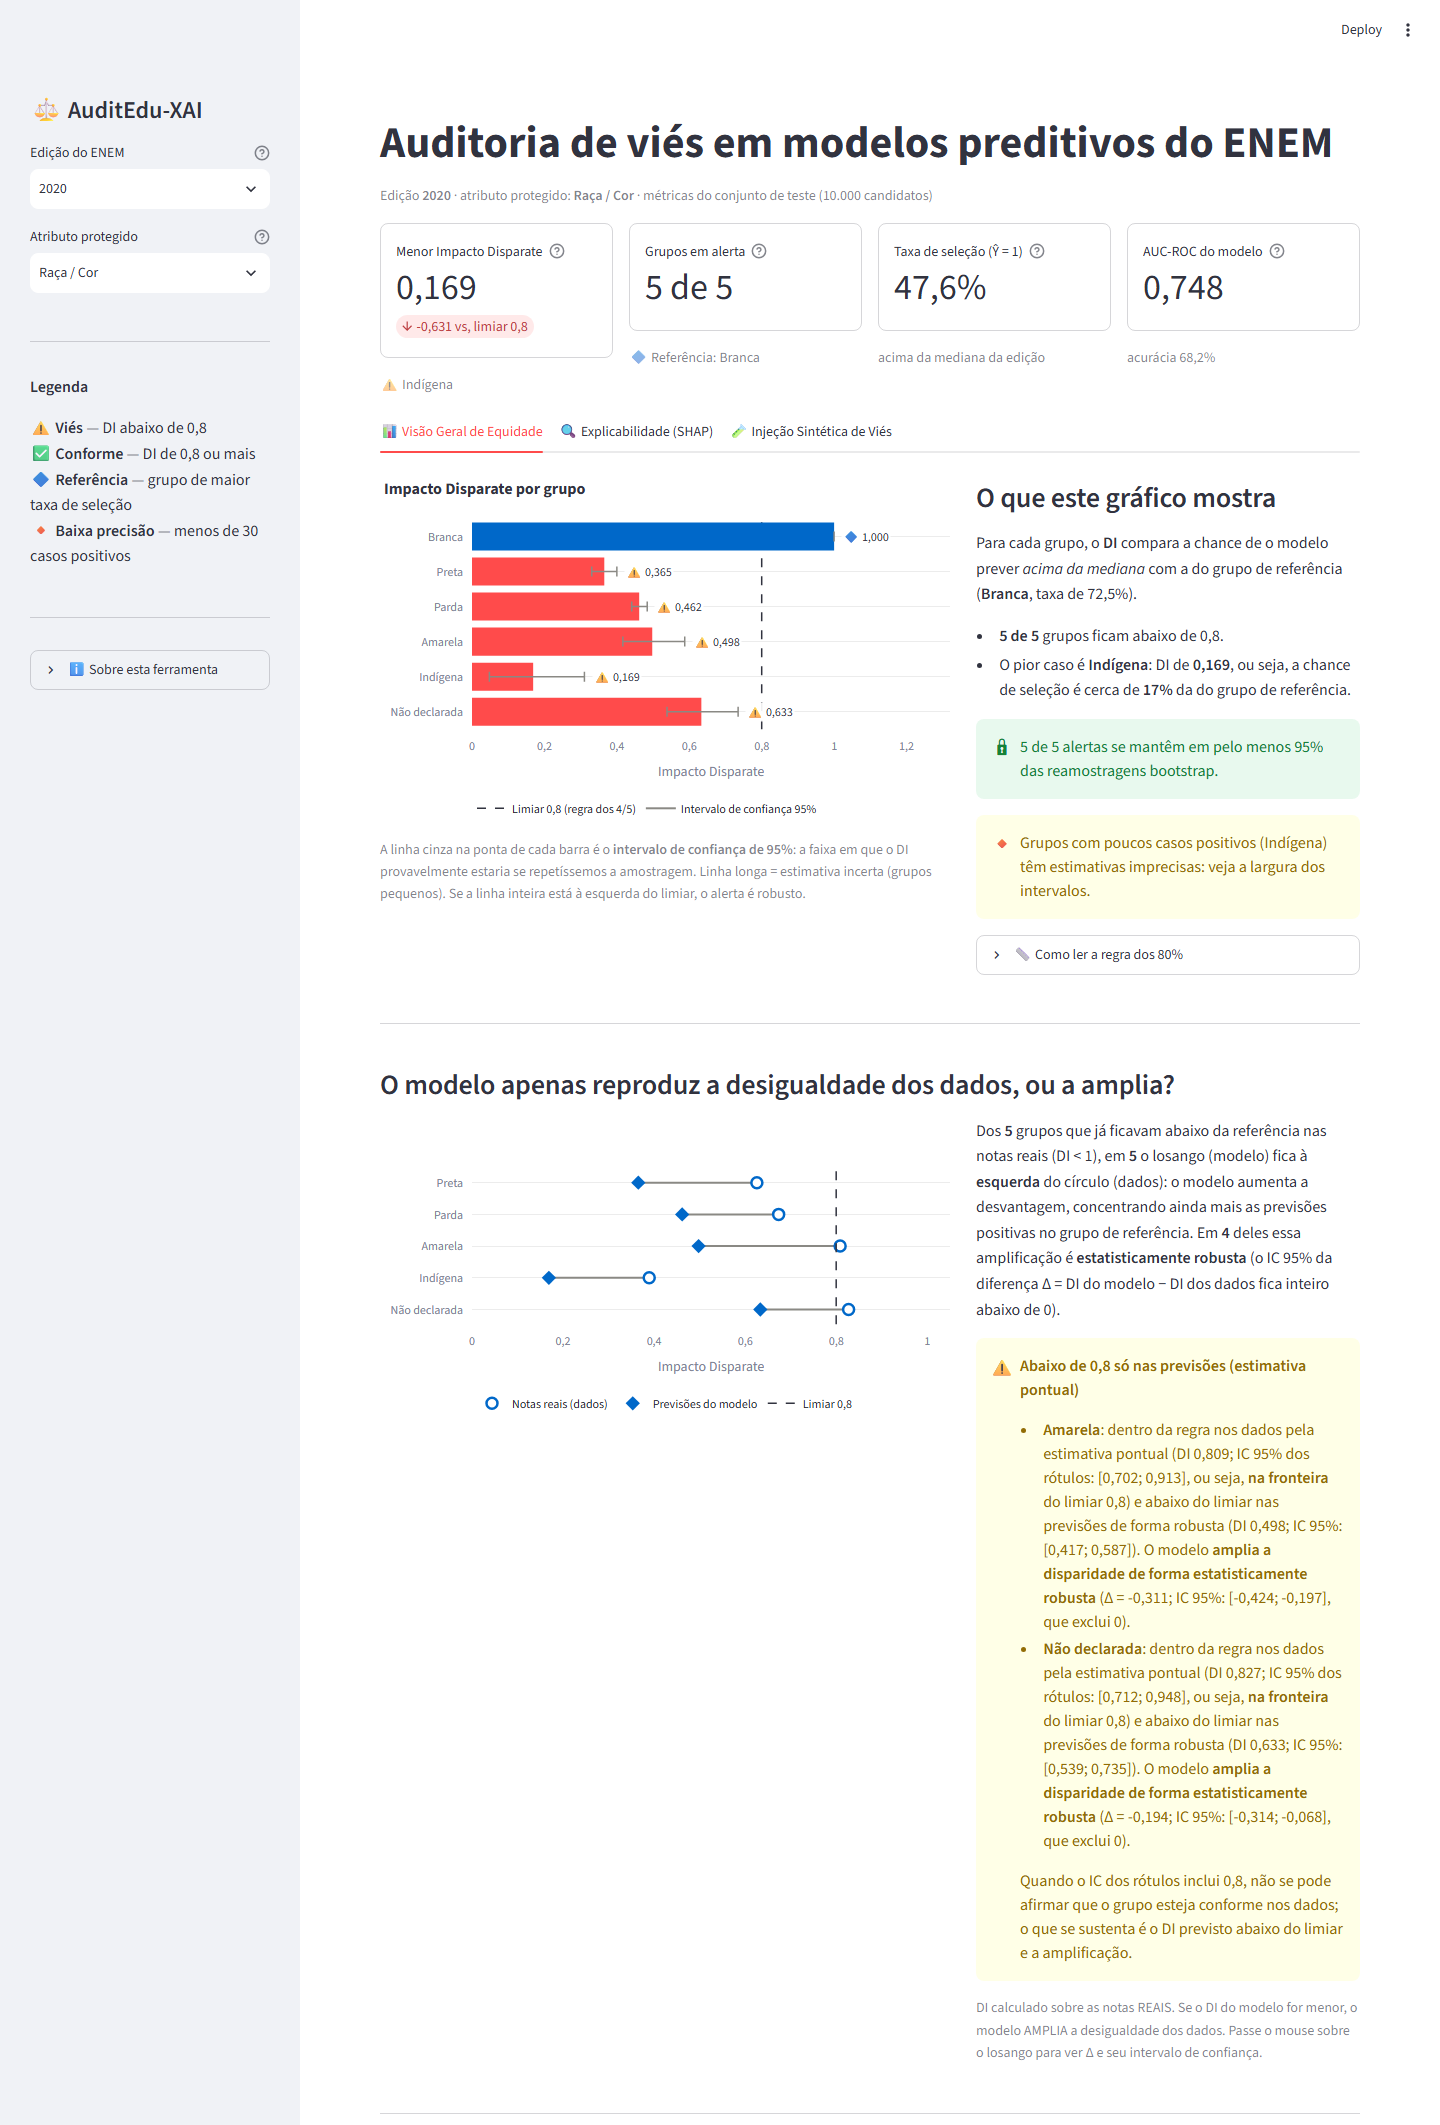
\includegraphics[width=\textwidth,trim=370 1727 70 215,clip]{../article/figuras/dashboard_equidade.png}\\[4pt]
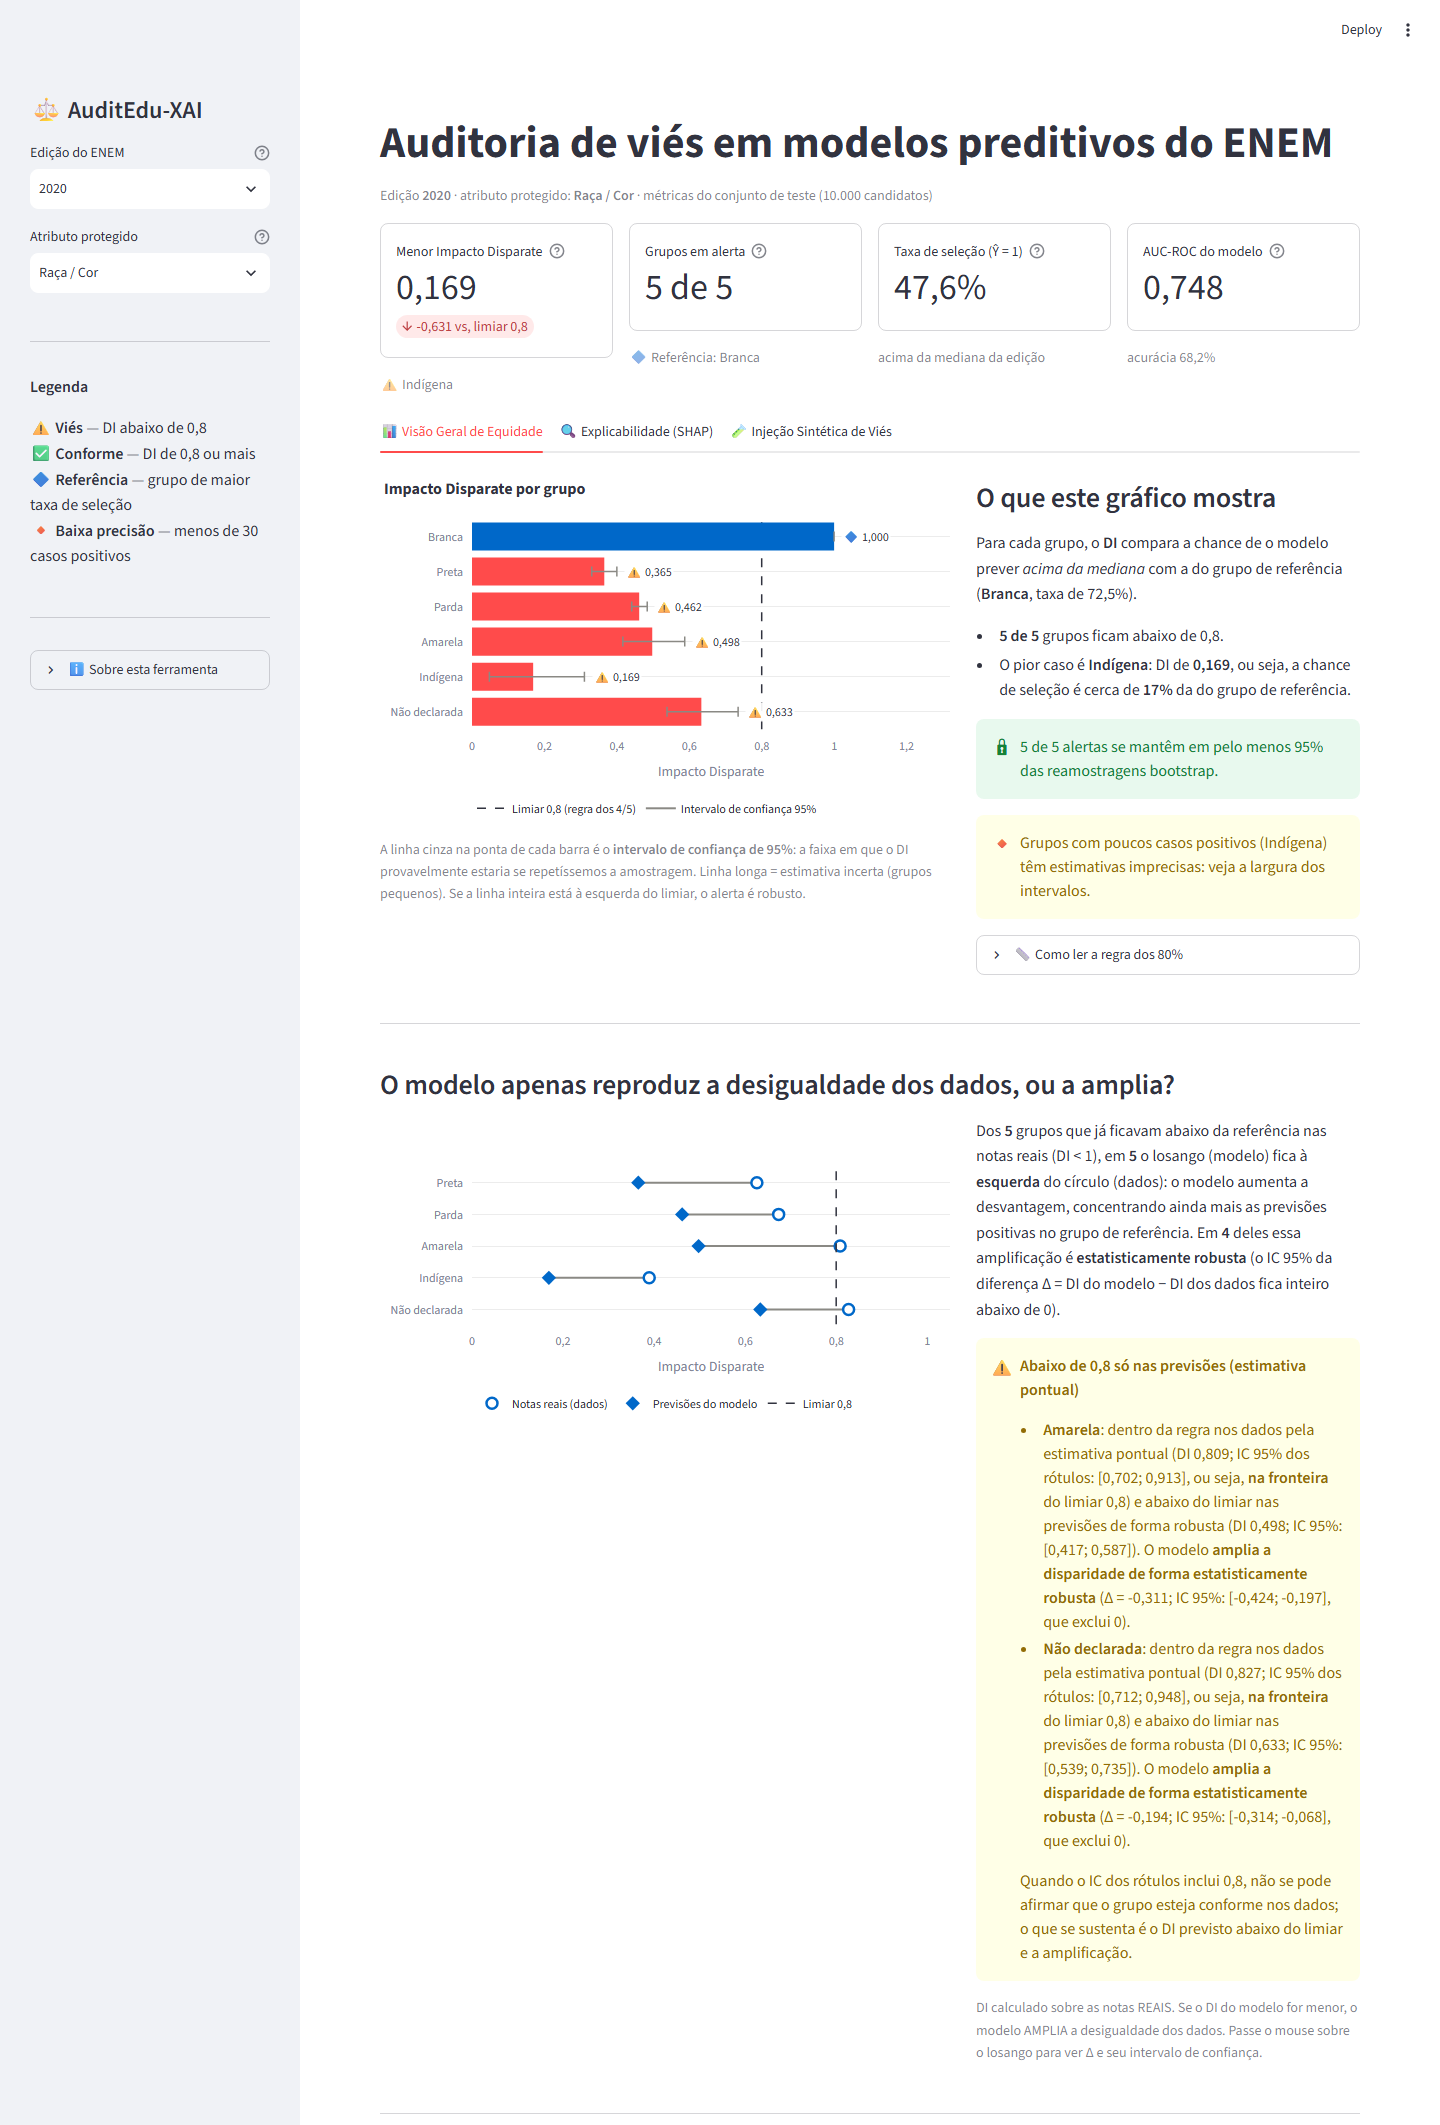
\includegraphics[width=0.8\textwidth,trim=375 1295 482 470,clip]{../article/figuras/dashboard_equidade.png}
\caption{Interface: indicadores e gráfico de DI da aba ``Visão Geral de Equidade'' (ENEM 2020, raça/cor; recortes da captura)}
\label{fig:dash_equidade}
\fonte{Elaborado pelos autores (captura da interface).}
\end{figure}

\subsection{Implantação, Desempenho e Reprodutibilidade}
\label{sec:implantacao}

A interface está implantada publicamente no Streamlit Community Cloud, serviço gratuito, em \url{https://auditeduxai.streamlit.app/}. A arquitetura desacoplada é o que viabiliza a hospedagem gratuita; como limitação operacional, aplicações sem acesso por 12 horas são hibernadas e demandam alguns segundos para reativação. A interface também é empacotada em uma imagem Docker de dois estágios, que contém apenas as dependências da interface, o código e os Parquets e executa como usuário não privilegiado. A imagem é validada por integração contínua (GitHub Actions) a cada alteração: o \textit{workflow} constrói a imagem, executa o contêiner limitado a 2 CPUs, aguarda o \textit{health check} e executa a interface completa em modo \textit{headless} para as três edições e os dois atributos, falhando se ocorrer qualquer exceção.

Os Parquets consumidos pela interface ocupam menos de 1~MB por edição, e dois níveis de cache evitam releituras e o redesenho do \textit{summary plot}, a operação mais cara da página, que por isso é exibido sob demanda. O tempo de resposta foi medido localmente executando a interface em modo \textit{headless} para cada edição e atributo (uma primeira carga e cinco interações), sem restrição e com a afinidade do processo restrita a 2 núcleos. Sem restrição, a primeira carga levou entre 0,17~s e 0,35~s; com 2 núcleos, entre 0,19~s e 0,33~s; nas duas configurações, as interações levaram em média entre 0,12~s e 0,19~s, com máximo de 0,280~s, e todas as 72 execuções ficaram abaixo de 2~s. A medição cobre a página na configuração padrão; a primeira renderização do \textit{summary plot}, acionada sob demanda, não está incluída. Essa medição é uma \textbf{aproximação} de um ambiente de nuvem com poucos núcleos, executada na mesma CPU física e sem a contenção de uma plataforma compartilhada; como a plataforma pública não divulga os recursos alocados, o tempo de resposta e o consumo de memória em produção não foram medidos.

Todas as etapas estocásticas usam a semente 42 ou geradores dela derivados, as versões das bibliotecas são fixadas, e um manifesto registra os \textit{hashes} SHA-256 dos dados, modelos e saídas. As tabelas e figuras de resultados deste artigo não são transcritas manualmente: um \textit{script} lê os Parquets e gera o código \LaTeX\ correspondente, de modo que qualquer divergência entre texto e artefato torna-se detectável.

\section{Resultados e Discussão}
\label{sec:resultados}

Todas as métricas desta seção foram calculadas exclusivamente sobre o conjunto de teste de cada edição ($n = 10.000$), e as tabelas e figuras são geradas automaticamente a partir dos arquivos Parquet do pipeline.

\subsection{Desempenho do Modelo-Alvo}
\label{sec:res_desempenho}

Nas três edições, a busca em grade selecionou a mesma configuração (100 árvores, profundidade máxima 3 e taxa de aprendizado 0,1), e o desempenho manteve-se estável: acurácia entre 0,6822 e 0,6842 e AUC-ROC entre 0,7475 e 0,7511 (Tabela~\ref{tab:desempenho}). Os três hiperparâmetros situam-se nos limites da grade, o que indica que uma grade mais ampla poderia produzir ganhos marginais, não perseguidos porque o modelo é o \textbf{objeto} da auditoria, e não o produto do trabalho. O F1 (entre 0,674 e 0,677) é inferior, mas da mesma ordem de grandeza, ao de \cite{luz2025uso} (0,758), que, porém, empregam mais variáveis e tomam como classe positiva o desempenho \textbf{abaixo} da média. Um modelo com AUC-ROC próxima de 0,75 seria considerado razoável em muitas aplicações, e é justamente esse tipo de modelo, aparentemente aceitável, que a ferramenta deve examinar.

% ARQUIVO GERADO AUTOMATICAMENTE por article/scripts/gerar_resultados.py
% Fonte: data/outputs/*.parquet — NÃO EDITAR À MÃO.
\begin{table}[htbp]
\centering
\caption{Desempenho do modelo-alvo (XGBoost) no conjunto de teste}
\label{tab:desempenho}
\resizebox{\textwidth}{!}{%
\begin{tabular}{lccccccc}
\toprule
\textbf{Edição} & \textbf{Acurácia} & \textbf{Precisão} & \textbf{Recall} & \textbf{F1} & \textbf{AUC-ROC} & \textbf{n\_est. / prof. / taxa} & \textbf{$n_{\text{teste}}$} \\
\midrule
2019 & 0,6842 & 0,7000 & 0,6490 & 0,6736 & 0,7511 & 100 / 3 / 0,10 & 10.000 \\
2020 & 0,6825 & 0,6926 & 0,6584 & 0,6751 & 0,7475 & 100 / 3 / 0,10 & 10.000 \\
2021 & 0,6822 & 0,6868 & 0,6673 & 0,6769 & 0,7480 & 100 / 3 / 0,10 & 10.000 \\
\bottomrule
\end{tabular}}
\fonte{\elaboradopor{} a partir de \texttt{model\_metrics\_\{ano\}.parquet}.}
\end{table}


\subsection{Equidade por Raça/Cor}
\label{sec:res_raca}

Em todas as edições, o grupo de referência é o de candidatos brancos, e \textbf{todos os grupos não brancos apresentam DI inferior a 0,8} (Tabela~\ref{tab:di_raca}). Os grupos Preta e Parda, que juntos representam mais da metade dos candidatos, apresentam as disparidades mais consistentes e com tendência de agravamento: o DI do grupo Preta passa de 0,426 em 2019 para 0,365 em 2020 e 0,337 em 2021, e o do grupo Parda, de 0,495 para 0,462 e 0,423. Em 2021, um candidato preto tinha cerca de um terço da probabilidade de um candidato branco de ser classificado acima da mediana.

% ARQUIVO GERADO AUTOMATICAMENTE por article/scripts/gerar_resultados.py
% Fonte: data/outputs/*.parquet — NÃO EDITAR À MÃO.
\begin{table}[htbp]
\centering
\caption{Impacto Disparate e Igualdade de Oportunidades por raça/cor no conjunto de teste, com intervalos de confiança de 95\%}
\label{tab:di_raca}
\resizebox{\textwidth}{!}{%
\begin{tabular}{lccccccc}
\toprule
\textbf{Grupo} & \textbf{$n$} & \textbf{$n$ ($Y=1$)} & \textbf{DI} & \textbf{IC95\% DI} & \textbf{TPR} & \textbf{IC95\% TPR} & \textbf{DI $<$ 0,8} \\
\midrule
\multicolumn{8}{l}{\textbf{ENEM 2019}} \\
\quad Branca (ref.) & 3.723 & 2.341 & 1,000 & -- & 0,801 & [0,784; 0,817] & Não \\
\quad Preta & 1.219 & 488 & 0,426 & [0,387; 0,465] & 0,469 & [0,424; 0,515] & \textbf{Sim} \\
\quad Parda & 4.581 & 1.954 & 0,495 & [0,472; 0,518] & 0,521 & [0,498; 0,542] & \textbf{Sim} \\
\quad Amarela & 225 & 106 & 0,609 & [0,517; 0,705] & 0,623 & [0,531; 0,710] & \textbf{Sim} \\
\quad Indígena & 52 & 19 & 0,252 & [0,115; 0,414] & 0,316 & [0,125; 0,545] & \textbf{Sim} \\
\quad Não declarada & 200 & 112 & 0,620 & [0,522; 0,720] & 0,580 & [0,491; 0,675] & \textbf{Sim} \\
\midrule
\multicolumn{8}{l}{\textbf{ENEM 2020}} \\
\quad Branca (ref.) & 3.793 & 2.386 & 1,000 & -- & 0,842 & [0,827; 0,856] & Não \\
\quad Preta & 1.227 & 483 & 0,365 & [0,331; 0,400] & 0,418 & [0,373; 0,460] & \textbf{Sim} \\
\quad Parda & 4.505 & 1.909 & 0,462 & [0,441; 0,484] & 0,505 & [0,483; 0,528] & \textbf{Sim} \\
\quad Amarela & 230 & 117 & 0,498 & [0,417; 0,587] & 0,496 & [0,406; 0,589] & \textbf{Sim} \\
\quad Indígena & 49 & 12 & 0,169 & [0,048; 0,310] & 0,167 & [0,000; 0,429] & \textbf{Sim} \\
\quad Não declarada & 196 & 102 & 0,633 & [0,539; 0,735] & 0,627 & [0,533; 0,726] & \textbf{Sim} \\
\midrule
\multicolumn{8}{l}{\textbf{ENEM 2021}} \\
\quad Branca (ref.) & 4.427 & 2.730 & 1,000 & -- & 0,830 & [0,816; 0,844] & Não \\
\quad Preta & 1.104 & 405 & 0,337 & [0,302; 0,373] & 0,343 & [0,298; 0,390] & \textbf{Sim} \\
\quad Parda & 4.022 & 1.643 & 0,423 & [0,401; 0,444] & 0,477 & [0,453; 0,501] & \textbf{Sim} \\
\quad Amarela & 211 & 109 & 0,663 & [0,570; 0,759] & 0,706 & [0,617; 0,792] & \textbf{Sim} \\
\quad Indígena & 47 & 9 & 0,417 & [0,231; 0,613] & 0,778 & [0,429; 1,000] & \textbf{Sim} \\
\quad Não declarada & 189 & 93 & 0,629 & [0,530; 0,731] & 0,602 & [0,500; 0,703] & \textbf{Sim} \\
\bottomrule
\end{tabular}}
\fonte{\elaboradopor{} a partir de \texttt{fairness\_metrics\_\{ano\}.parquet}. Grupo de referência: maior taxa de seleção. IC95\%: percentis 2,5 e 97,5 de 2.000 reamostragens \textit{bootstrap} do conjunto de teste, com o modelo fixo. A FPR por grupo é apresentada na Figura~\ref{fig:tpr_fpr}.}
\end{table}


O \textbf{alerta é estatisticamente robusto para todos os grupos não brancos}, inclusive o Indígena: o limite superior do IC95\% do DI não ultrapassa 0,759 em nenhum caso, e em ao menos 99,5\% das reamostragens o DI permaneceu abaixo de 0,8. A tendência de agravamento dos grupos Preta e Parda também é sustentada, pois os intervalos de 2019 e 2021 não se sobrepõem. Já o grupo Indígena conta com apenas 47 a 52 candidatos no teste, e \textbf{suas estimativas de TPR não são conclusivas}: com 19, 12 e 9 rótulos positivos, os intervalos são muito amplos ([0,000; 0,429] em 2020 e [0,429; 1,000] em 2021), e a TPR de 0,778 em 2021 não deve ser lida como evidência de igualdade de oportunidades; a variação abrupta do DI indígena em 2021 (0,417) é compatível com flutuação amostral.

O modelo também \textbf{erra de forma assimétrica} (Figura~\ref{fig:tpr_fpr}). Entre os candidatos com NMG igual ou superior à mediana, reconhece entre 80,1\% e 84,2\% dos brancos, mas apenas 46,9\%, 41,8\% e 34,3\% dos pretos em 2019, 2020 e 2021, e entre 47,7\% e 52,1\% dos pardos. Simetricamente, a FPR de candidatos brancos (0,492 a 0,530) é cerca de três vezes a de pretos (0,165 a 0,182). O modelo concede mais classificações acima da mediana indevidas ao grupo privilegiado e nega mais classificações merecidas aos grupos protegidos, violando os critérios de \textit{Equal Opportunity} e \textit{Equalized Odds}.

\begin{figure}[htbp]
\centering
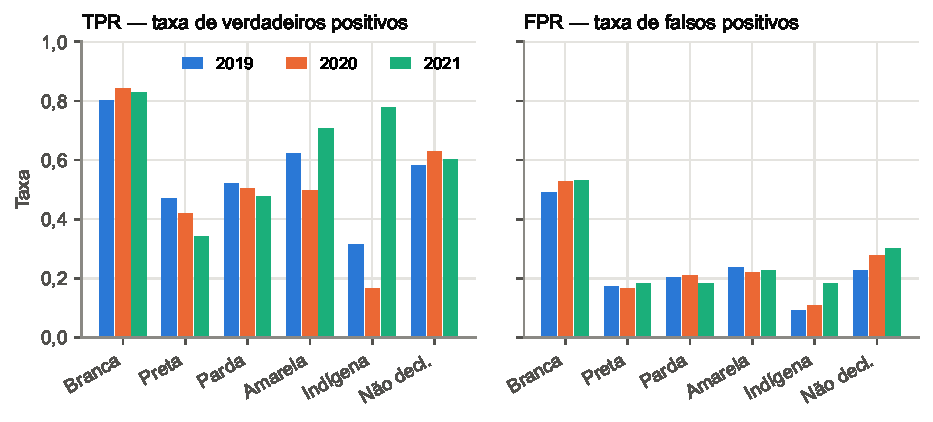
\includegraphics[width=0.85\textwidth]{../article/figuras/resultados/fig_tpr_fpr_raca.pdf}
\caption{Taxas de verdadeiros positivos (TPR) e de falsos positivos (FPR) por raça/cor}
\label{fig:tpr_fpr}
\fonte{Elaborado pelos autores a partir de \texttt{fairness\_metrics\_\{ano\}.parquet}.}
\end{figure}

\subsection{Equidade por Renda Familiar}
\label{sec:res_renda}

A renda familiar produz o gradiente mais acentuado (Tabela~\ref{tab:di_renda}). Nas três edições, \textbf{as faixas A a E (até 2,5 salários mínimos) violam a regra dos quatro quintos}, e as faixas A e B têm DI entre 0,044 e 0,074: o modelo praticamente nunca classifica esses candidatos acima da mediana. Na faixa B, a TPR é de apenas 0,077, 0,126 e 0,115 em 2019, 2020 e 2021, ou seja, quase nove em cada dez candidatos de baixa renda que superaram a mediana são classificados incorretamente. A fronteira do alerta situa-se entre as faixas E e F. Na faixa E, o DI fica abaixo de 0,8 em pelo menos 98\% das reamostragens nas três edições; já a faixa F em 2021 ($\mathrm{DI} = 0{,}803$, IC95\% [0,774; 0,832]) encontra-se \textbf{sobre o limiar}, com DI abaixo de 0,8 em 41,2\% das reamostragens, e a ausência de alerta não deve ser lida como conformidade. Como várias faixas superiores empatam com taxas de seleção próximas de 100\%, a referência varia entre as edições (L, J e L), sem impacto relevante sobre as faixas inferiores; e, como os limites das faixas são expressos em salários mínimos de cada ano, a comparação entre edições é relativa.

% ARQUIVO GERADO AUTOMATICAMENTE por article/scripts/gerar_resultados.py
% Fonte: data/outputs/*.parquet — NÃO EDITAR À MÃO.
\begin{table}[htbp]
\centering
\caption{Impacto Disparate e TPR por faixa de renda familiar (Q006) no conjunto de teste}
\label{tab:di_renda}
\begin{tabular}{llcccccc}
\toprule
 & & \multicolumn{3}{c}{\textbf{DI}} & \multicolumn{3}{c}{\textbf{TPR}} \\
\cmidrule(lr){3-5}\cmidrule(lr){6-8}
\textbf{Faixa} & \textbf{Renda mensal} & 2019 & 2020 & 2021 & 2019 & 2020 & 2021 \\
\midrule
A & Nenhuma renda & \textbf{0,070} & \textbf{0,072} & \textbf{0,044} & 0,190 & 0,181 & 0,108 \\
B & Até 1 SM & \textbf{0,047} & \textbf{0,074} & \textbf{0,053} & 0,077 & 0,126 & 0,115 \\
C & 1 a 1,5 SM & \textbf{0,209} & \textbf{0,356} & \textbf{0,207} & 0,284 & 0,447 & 0,290 \\
D & 1,5 a 2 SM & \textbf{0,662} & \textbf{0,569} & \textbf{0,481} & 0,736 & 0,664 & 0,575 \\
E & 2 a 2,5 SM & \textbf{0,771} & \textbf{0,764} & \textbf{0,723} & 0,858 & 0,827 & 0,767 \\
F & 2,5 a 3 SM & 0,848 & 0,855 & 0,803 & 0,884 & 0,883 & 0,869 \\
G & 3 a 4 SM & 0,897 & 0,947 & 0,883 & 0,921 & 0,961 & 0,911 \\
H & 4 a 5 SM & 0,976 & 0,982 & 0,938 & 0,983 & 0,989 & 0,961 \\
I & 5 a 6 SM & 0,968 & 0,983 & 0,974 & 0,981 & 0,984 & 0,973 \\
J & 6 a 7 SM & 0,995 & 1,000 & 0,990 & 0,994 & 1,000 & 0,987 \\
K & 7 a 8 SM & 0,986 & 0,992 & 0,981 & 1,000 & 1,000 & 0,991 \\
L & 8 a 9 SM & 1,000 & 1,000 & 1,000 & 1,000 & 1,000 & 1,000 \\
M & 9 a 10 SM & 0,989 & 1,000 & 0,986 & 0,987 & 1,000 & 0,988 \\
N & 10 a 12 SM & 1,000 & 1,000 & 0,993 & 1,000 & 1,000 & 0,991 \\
O & 12 a 15 SM & 0,990 & 1,000 & 0,992 & 1,000 & 1,000 & 0,991 \\
P & 15 a 20 SM & 1,000 & 0,991 & 0,985 & 1,000 & 1,000 & 0,991 \\
Q & Acima de 20 SM & 1,000 & 1,000 & 1,000 & 1,000 & 1,000 & 1,000 \\
\bottomrule
\end{tabular}
\fonte{\elaboradopor{} a partir de \texttt{fairness\_metrics\_\{ano\}.parquet}. SM = salário mínimo vigente no ano. Em negrito: DI $<$ 0,8. Faixa de referência (maior taxa de seleção) --- 2019: L, 2020: J, 2021: L.}
\end{table}


\subsection{Amplificação do Viés pelo Modelo}
\label{sec:res_amplificacao}

A Tabela~\ref{tab:amplificacao} compara o DI dos rótulos reais com o das predições (Equação~\ref{eq:amplificacao}). Em 14 das 15 combinações de grupo e edição, o DI das predições é inferior ao dos rótulos, com reduções entre 0,140 e 0,329, e em 13 delas o IC95\% de $\Delta_g$ fica inteiramente abaixo de zero. As duas exceções são do grupo Indígena: em 2020, a estimativa é negativa ($-0{,}220$), mas o intervalo inclui zero; em 2021, $\Delta_g = +0{,}106$, com intervalo [$-0{,}070$; 0,296]. Para esse grupo, a amplificação só é sustentada em 2019, e nem a amplificação de 2020 nem a atenuação de 2021 podem ser distinguidas de zero.

% ARQUIVO GERADO AUTOMATICAMENTE por article/scripts/gerar_resultados.py
% Fonte: data/outputs/*.parquet — NÃO EDITAR À MÃO.
\begin{table}[htbp]
\centering
\caption{Impacto Disparate dos rótulos reais ($y$) versus das predições ($\hat{y}$) por raça/cor, com intervalos de confiança de 95\%}
\label{tab:amplificacao}
\begin{tabular}{lccccc}
\toprule
\textbf{Grupo} & $\mathrm{DI}_y$ & \textbf{IC95\%} $\mathrm{DI}_y$ & $\mathrm{DI}_{\hat{y}}$ & $\Delta$ & \textbf{IC95\%} $\Delta$ \\
\midrule
\multicolumn{6}{l}{\textbf{ENEM 2019}} \\
\quad Preta & 0,637 & [0,590; 0,684] & 0,426 & \textbf{−0,211} & [−0,264; −0,160] \\
\quad Parda & 0,678 & [0,650; 0,707] & 0,495 & \textbf{−0,183} & [−0,214; −0,153] \\
\quad Amarela & 0,749 & [0,644; 0,852] & 0,609 & \textbf{−0,140} & [−0,253; −0,032] \\
\quad Indígena & 0,581 & [0,368; 0,802] & 0,252 & \textbf{−0,329} & [−0,570; −0,100] \\
\quad Não declarada & 0,891 & [0,775; 1,002] & 0,620 & \textbf{−0,271} & [−0,393; −0,145] \\
\midrule
\multicolumn{6}{l}{\textbf{ENEM 2020}} \\
\quad Preta & 0,626 & [0,578; 0,670] & 0,365 & \textbf{−0,260} & [−0,309; −0,209] \\
\quad Parda & 0,674 & [0,645; 0,704] & 0,462 & \textbf{−0,212} & [−0,242; −0,184] \\
\quad Amarela & 0,809 & [0,702; 0,913] & 0,498 & \textbf{−0,311} & [−0,424; −0,197] \\
\quad Indígena & 0,389 & [0,203; 0,588] & 0,169 & −0,220 & [−0,443; 0,008] \\
\quad Não declarada & 0,827 & [0,712; 0,948] & 0,633 & \textbf{−0,194} & [−0,314; −0,068] \\
\midrule
\multicolumn{6}{l}{\textbf{ENEM 2021}} \\
\quad Preta & 0,595 & [0,547; 0,643] & 0,337 & \textbf{−0,258} & [−0,310; −0,203] \\
\quad Parda & 0,662 & [0,632; 0,692] & 0,423 & \textbf{−0,240} & [−0,270; −0,208] \\
\quad Amarela & 0,838 & [0,723; 0,945] & 0,663 & \textbf{−0,175} & [−0,277; −0,066] \\
\quad Indígena & 0,311 & [0,136; 0,503] & 0,417 & +0,106 & [−0,070; 0,296] \\
\quad Não declarada & 0,798 & [0,675; 0,910] & 0,629 & \textbf{−0,169} & [−0,294; −0,042] \\
\bottomrule
\end{tabular}
\fonte{\elaboradopor{} a partir de \texttt{fairness\_metrics\_\{ano\}.parquet}. Referência: Branca. $\Delta = \mathrm{DI}_{\hat{y}} - \mathrm{DI}_y$ (valores negativos indicam amplificação da disparidade pelo modelo). Em negrito: $\Delta$ cujo IC95\% não inclui zero. IC95\%: percentis 2,5 e 97,5 das mesmas 2.000 reamostragens \textit{bootstrap} da Tabela~\ref{tab:di_raca}, com o modelo e o grupo de referência fixos. O IC95\% de $\mathrm{DI}_{\hat{y}}$ consta da Tabela~\ref{tab:di_raca}.}
\end{table}


O caso mais revelador é o de grupos cujo DI nos rótulos está \textbf{na fronteira do limiar} (não declarada em 2019 e 2020; amarela em 2020 e 2021): a estimativa pontual de $\mathrm{DI}_y$ está em 0,8 ou acima, mas o intervalo inclui 0,8, ao passo que o DI das predições tem IC95\% inteiramente abaixo de 0,8 e a amplificação, IC95\% inteiramente negativo. O modelo \textbf{desloca esses grupos de uma situação de fronteira para uma posição claramente abaixo do limiar}. Um mecanismo plausível é o limiar de decisão: quando a maior parte dos perfis de um grupo tem probabilidade estimada inferior a 0,5, o modelo atribui a classe negativa a quase todos os seus membros, comprimindo a taxa de seleção abaixo da taxa-base real.

Na renda, a amplificação com desvantagem para a faixa é robusta nas faixas mais baixas, A, B e C, nas três edições ($\Delta$ entre $-0{,}322$ e $-0{,}178$), e D em 2021 ($\Delta = -0{,}120$; IC95\% [$-0{,}187$; $-0{,}062$]), e nas faixas intermediárias os intervalos incluem zero na maioria dos casos\footnote{\raggedright Os valores de $\Delta$ por faixa e edição, com IC95\%, estão nos arquivos \texttt{fairness\_metrics\_\{ano\}.parquet} do repositório público do artefato, \url{https://github.com/rbrtotavio/audit_edu_xai}.}. Nas faixas superiores, valores negativos de $\Delta$ são \textbf{mecânicos}: como $\mathrm{DI}_{\hat{y}} \leq 1$ por construção, quando $\mathrm{DI}_y > 1$ o valor $\Delta < 0$ reflete a aproximação do DI previsto ao da faixa de referência, e não desvantagem para essas faixas.

\subsection{Explicabilidade: Fatores Determinantes}
\label{sec:res_shap}

A Tabela~\ref{tab:shap} apresenta o ranking de importância global SHAP. Primeiro, \textbf{a ausência de computador na residência (Q024 = A) é o atributo mais influente nas três edições}, e sua importância média cresce de 0,405 em 2019 para 0,448 em 2020 e 0,506 em 2021, um aumento de 25\%; a categoria ``um computador'' sobe da quinta posição (0,095) para a segunda (0,203). O crescimento coincide temporalmente com o ensino remoto emergencial da pandemia de COVID-19 e é \textbf{compatível} com a hipótese de agravamento da exclusão digital, mas o desenho observacional e sem grupo de comparação \textbf{não permite atribuí-lo causalmente à pandemia}. Além disso, os valores SHAP descrevem o comportamento do modelo, e não relações causais, e a composição dos participantes mudou (de 3,70 milhões de presentes em 2019 para 2,24 milhões em 2021).

% ARQUIVO GERADO AUTOMATICAMENTE por article/scripts/gerar_resultados.py
% Fonte: data/outputs/*.parquet — NÃO EDITAR À MÃO.
\begin{table}[htbp]
\centering
\caption{Ranking de importância global SHAP (média de $|\phi_i|$, escala log-odds) no conjunto de teste}
\label{tab:shap}
\resizebox{\textwidth}{!}{%
\begin{tabular}{clclclc}
\toprule
 & \multicolumn{2}{c}{\textbf{2019}} & \multicolumn{2}{c}{\textbf{2020}} & \multicolumn{2}{c}{\textbf{2021}} \\
\cmidrule(lr){2-3}\cmidrule(lr){4-5}\cmidrule(lr){6-7}
\textbf{\#} & \textbf{Atributo} & $\overline{|\phi|}$ & \textbf{Atributo} & $\overline{|\phi|}$ & \textbf{Atributo} & $\overline{|\phi|}$ \\
\midrule
1 & Computador: nenhum computador & 0,405 & Computador: nenhum computador & 0,448 & Computador: nenhum computador & 0,506 \\
2 & Renda: até 1 SM & 0,186 & Renda: até 1 SM & 0,194 & Computador: um computador & 0,203 \\
3 & Renda: 1 a 1,5 SM & 0,134 & Raça/cor: branca & 0,164 & Renda: até 1 SM & 0,181 \\
4 & Raça/cor: branca & 0,130 & Computador: um computador & 0,137 & Raça/cor: branca & 0,148 \\
5 & Computador: um computador & 0,095 & Renda: 1 a 1,5 SM & 0,085 & Renda: 1 a 1,5 SM & 0,082 \\
6 & Escol. da mãe: superior completo & 0,083 & Renda: nenhuma renda & 0,075 & Escol. do pai: superior completo & 0,077 \\
7 & Escol. da mãe: médio completo & 0,081 & Escol. do pai: médio completo & 0,071 & Escol. do pai: médio completo & 0,073 \\
8 & Escol. da mãe: pós-graduação & 0,075 & Escol. da mãe: médio completo & 0,068 & Renda: nenhuma renda & 0,065 \\
\bottomrule
\end{tabular}}
\fonte{\elaboradopor{} a partir de \texttt{shap\_values\_\{ano\}.parquet}.}
\end{table}


Como a importância média de uma variável indicadora depende também de sua \textbf{prevalência}, o aumento poderia refletir apenas a proporção de candidatos sem computador. A Tabela~\ref{tab:shap_q024} não sustenta essa explicação: a prevalência no teste \textbf{diminuiu} de 0,445 em 2019 para 0,381 em 2021, enquanto a diferença entre a contribuição SHAP média de quem possui e de quem não possui computador \textbf{aumentou} de 0,830 para 1,116 log-odds (34\%). O peso atribuído à ausência de computador cresceu, portanto, por candidato, o que não exclui que a mudança no perfil dos participantes tenha alterado a própria associação aprendida. A queda da prevalência em 2021 é coerente com a redução do número de participantes e com a hipótese de que candidatos mais vulneráveis deixaram de realizar o exame.

% ARQUIVO GERADO AUTOMATICAMENTE por article/scripts/gerar_resultados.py
% Fonte: data/outputs/*.parquet — NÃO EDITAR À MÃO.
\begin{table}[htbp]
\centering
\caption{Decomposição da importância SHAP do atributo ``sem computador'' (Q024 = A) por edição}
\label{tab:shap_q024}
\begin{tabular}{cccccc}
\toprule
\textbf{Edição} & \textbf{Prevalência} & $\overline{|\phi|}$ & $\bar{\phi}$ \textbf{(sem comp.)} & $\bar{\phi}$ \textbf{(com comp.)} & \textbf{Diferença} \\
\midrule
2019 & 0,445 & 0,405 & −0,505 & 0,325 & 0,830 \\
2020 & 0,444 & 0,448 & −0,564 & 0,356 & 0,920 \\
2021 & 0,381 & 0,506 & −0,774 & 0,342 & 1,116 \\
\bottomrule
\end{tabular}
\fonte{\elaboradopor{} a partir de \texttt{shap\_feature\_summary\_\{ano\}.parquet}. Prevalência: proporção de candidatos sem computador no teste. Diferença: $\bar{\phi}$ (com comp.) $-$ $\bar{\phi}$ (sem comp.), em log-odds.}
\end{table}


Segundo, \textbf{a faixa de renda de até 1 salário mínimo} (Q006~=~B) mantém-se entre os três atributos mais relevantes, ao lado das demais faixas inferiores de renda e da escolaridade dos pais, em consonância com a literatura \cite{souza2025desigualdades}. Terceiro, \textbf{a raça/cor branca figura entre os quatro atributos mais importantes em todas as edições}: mesmo dispondo de renda, escolaridade dos pais e acesso a tecnologia, o modelo usa diretamente a raça/cor como sinal preditivo, constatação que as métricas de equidade sozinhas não permitiriam estabelecer.

\subsection{Validação por Injeção Sintética de Viés}
\label{sec:res_injecao}

As Tabelas~\ref{tab:injecao} e~\ref{tab:injecao_efeito} apresentam a curva de sensibilidade e o efeito com 50\% de intensidade.

% ARQUIVO GERADO AUTOMATICAMENTE por article/scripts/gerar_resultados.py
% Fonte: data/outputs/*.parquet — NÃO EDITAR À MÃO.
\begin{table}[htbp]
\centering
\caption{Curva de sensibilidade: DI médio do grupo-alvo e AUC-ROC sob injeção sintética de viés (teste)}
\label{tab:injecao}
\resizebox{\textwidth}{!}{%
\begin{tabular}{l*{9}{c}}
\toprule
 & \multicolumn{3}{c}{\textbf{2019}} & \multicolumn{3}{c}{\textbf{2020}} & \multicolumn{3}{c}{\textbf{2021}} \\
\cmidrule(lr){2-4}\cmidrule(lr){5-7}\cmidrule(lr){8-10}
\textbf{Intensidade $p$} & DI (injeção) & DI (controle) & AUC & DI (injeção) & DI (controle) & AUC & DI (injeção) & DI (controle) & AUC \\
\midrule
\multicolumn{10}{l}{\textbf{Grupo-alvo: Parda}} \\
\quad 0\% & 0,495 $\pm$ 0,000 & 0,495 & 0,751 & 0,462 $\pm$ 0,000 & 0,462 & 0,748 & 0,423 $\pm$ 0,000 & 0,423 & 0,748 \\
\quad 10\% & 0,384 $\pm$ 0,006 & 0,448 & 0,750 & 0,372 $\pm$ 0,007 & 0,434 & 0,746 & 0,344 $\pm$ 0,014 & 0,421 & 0,747 \\
\quad 25\% & 0,189 $\pm$ 0,011 & 0,432 & 0,743 & 0,184 $\pm$ 0,004 & 0,412 & 0,739 & 0,165 $\pm$ 0,001 & 0,405 & 0,740 \\
\quad 50\% & 0,005 $\pm$ 0,002 & 0,325 & 0,719 & 0,008 $\pm$ 0,005 & 0,318 & 0,717 & 0,005 $\pm$ 0,003 & 0,302 & 0,721 \\
\midrule
\multicolumn{10}{l}{\textbf{Grupo-alvo: Indígena}} \\
\quad 0\% & 0,252 $\pm$ 0,000 & 0,252 & 0,751 & 0,169 $\pm$ 0,000 & 0,169 & 0,748 & 0,417 $\pm$ 0,000 & 0,417 & 0,748 \\
\quad 10\% & 0,207 $\pm$ 0,015 & 0,257 & 0,751 & 0,152 $\pm$ 0,025 & 0,197 & 0,748 & 0,380 $\pm$ 0,013 & 0,419 & 0,748 \\
\quad 25\% & 0,190 $\pm$ 0,024 & 0,257 & 0,751 & 0,118 $\pm$ 0,012 & 0,186 & 0,748 & 0,250 $\pm$ 0,054 & 0,419 & 0,748 \\
\quad 50\% & 0,072 $\pm$ 0,015 & 0,256 & 0,751 & 0,079 $\pm$ 0,024 & 0,197 & 0,748 & 0,066 $\pm$ 0,039 & 0,417 & 0,748 \\
\bottomrule
\end{tabular}}
\fonte{\elaboradopor{} a partir de \texttt{bias\_injection\_summary.parquet}. Média $\pm$ desvio-padrão de 5 repetições. AUC do cenário de injeção.}
\end{table}


\textbf{Sensibilidade (H1).} Nas seis combinações de grupo e edição, o DI médio decresce estritamente a cada aumento da intensidade. Com 50\%, o DI do grupo Parda cai de 0,495 para 0,005 em 2019, de 0,462 para 0,008 em 2020 e de 0,423 para 0,005 em 2021 (o modelo quase deixa de selecionar pardos), e o do Indígena, de 0,252 para 0,072, de 0,169 para 0,079 e de 0,417 para 0,066. O desvio-padrão máximo de 0,014 entre repetições no grupo Parda indica resposta estável, e H1 é corroborada.

\textbf{Especificidade (H2).} No grupo Indígena, o controle praticamente não altera o DI (+0,004, +0,029 e +0,001 com 50\%). No grupo Parda, o controle também o reduz ($-0{,}170$, $-0{,}144$ e $-0{,}121$), porque o volume de rótulos alterados é elevado (até 3.916, cerca de um quinto dos positivos do treino) e desloca para baixo a probabilidade estimada de todos os candidatos, afetando primeiro os grupos próximos do limiar de decisão. Ainda assim, o efeito líquido (Equação~\ref{eq:efeito_liquido}) é negativo em todas as combinações de grupo, edição e intensidade; com 50\%, fica entre $-0{,}297$ e $-0{,}320$ para o grupo Parda e entre $-0{,}119$ e $-0{,}351$ para o Indígena, e H2 é corroborada.

% ARQUIVO GERADO AUTOMATICAMENTE por article/scripts/gerar_resultados.py
% Fonte: data/outputs/*.parquet — NÃO EDITAR À MÃO.
\begin{table}[htbp]
\centering
\caption{Efeito da injeção de 50\% de viés sobre os indicadores do artefato}
\label{tab:injecao_efeito}
\resizebox{\textwidth}{!}{%
\begin{tabular}{lcccccccc}
\toprule
\textbf{Grupo} & \textbf{Edição} & \textbf{Rótulos alterados} & $\Delta\mathrm{DI}_{\text{inj}}$ & $\Delta\mathrm{DI}_{\text{ctrl}}$ & \textbf{Efeito líquido} & $\Delta\mathrm{AUC}$ & \textbf{TPR (0\%$\rightarrow$50\%)} & $\bar{\phi}_{\text{raça}}$ \textbf{(0\%$\rightarrow$50\%)} \\
\midrule
Parda & 2019 & 3.916 & −0,490 & −0,170 & −0,320 & −0,032 & 0,521 $\rightarrow$ 0,007 & −0,004 $\rightarrow$ −0,509 \\
Parda & 2020 & 3.826 & −0,454 & −0,144 & −0,310 & −0,031 & 0,505 $\rightarrow$ 0,012 & −0,002 $\rightarrow$ −0,421 \\
Parda & 2021 & 3.334 & −0,418 & −0,121 & −0,297 & −0,027 & 0,477 $\rightarrow$ 0,007 & 0,000 $\rightarrow$ −0,452 \\
Indígena & 2019 & 34 & −0,180 & +0,004 & −0,184 & 0,000 & 0,316 $\rightarrow$ 0,126 & −0,227 $\rightarrow$ −1,062 \\
Indígena & 2020 & 24 & −0,090 & +0,029 & −0,119 & 0,000 & 0,167 $\rightarrow$ 0,183 & −0,461 $\rightarrow$ −1,217 \\
Indígena & 2021 & 24 & −0,350 & +0,001 & −0,351 & 0,000 & 0,778 $\rightarrow$ 0,089 & −0,144 $\rightarrow$ −0,939 \\
\bottomrule
\end{tabular}}
\fonte{\elaboradopor{} a partir de \texttt{bias\_injection\_summary.parquet}. $\bar{\phi}_{\text{raça}}$: valor SHAP médio da variável indicadora do grupo-alvo entre os membros do grupo.}
\end{table}


\textbf{Baixa sensibilidade das métricas convencionais (H3).} Com 50\% de injeção no grupo Parda, o DI despenca para valores entre 0,005 e 0,008, enquanto \textbf{a AUC-ROC recua, em média, apenas entre 0,027 e 0,032}, permanecendo acima de 0,71. Para o grupo Indígena, que representa cerca de 0,5\% do teste, \textbf{a AUC-ROC não se altera na terceira casa decimal}, embora o DI recue entre 53\% e 84\%. A AUC-ROC não fica rigorosamente constante; o ponto é a \textbf{desproporção}: uma validação baseada apenas em métricas convencionais poderia aprovar um modelo que exclui sistematicamente candidatos pardos ou indígenas. O artefato detecta o viés por três vias: o \textbf{DI}, que dispara o alerta e cai com a intensidade; a \textbf{TPR}, que no grupo Parda cai de cerca de 0,5 para valores entre 0,007 e 0,012 (no grupo Indígena, o leve aumento em 2020, de 0,167 para 0,183, reflete a flutuação amostral de um grupo pequeno); e os \textbf{valores SHAP}, que \textbf{localizam a origem do viés}: o SHAP médio da indicadora ``raça/cor parda'' entre os candidatos pardos passa de aproximadamente zero para valores entre $-0{,}421$ e $-0{,}509$, e o da indicadora ``raça/cor indígena'' entre os indígenas, de $-0{,}144$ a $-0{,}461$ para $-0{,}939$ a $-1{,}217$. O modelo passou a penalizar diretamente o pertencimento ao grupo, e H3 é corroborada.

\section{Conclusão}
\label{sec:conclusao}

Este artigo apresentou o AuditEdu-XAI, ferramenta de auditoria algorítmica projetada, desenvolvida e avaliada segundo a DSR, que integra métricas de justiça algorítmica e explicações SHAP em uma arquitetura desacoplada executável em infraestrutura gratuita. A resposta à questão de pesquisa é afirmativa, com as ressalvas apontadas a seguir: a ferramenta detectou, quantificou e explicou vieses de raça/cor e renda em modelos preditivos do ENEM e mostrou-se sensível a vieses aos quais a AUC-ROC pouco respondeu.

A contribuição \textbf{tecnológica} é um artefato, com código publicado em repositório público, que combina métricas de equidade de grupo, decomposição do viés entre dados e modelo, explicações TreeSHAP e uma interface acessível a usuários sem formação em programação; sua implantação pública demonstra que a auditoria algorítmica pode ser oferecida sem custo de infraestrutura, em um padrão potencialmente replicável para outras bases públicas. A contribuição \textbf{empírica} reúne três achados: um modelo de desempenho moderado viola a regra dos quatro quintos para todos os grupos não brancos e para candidatos com renda familiar de até 2,5 salários mínimos, nas três edições; o modelo \textbf{amplifica} a disparidade dos dados, de forma estatisticamente robusta em 13 das 15 combinações de raça/cor e edição e nas faixas de renda mais baixas, levando para baixo do limiar grupos cujo DI nos rótulos estava na fronteira de 0,8; e a ausência de computador na residência é o atributo mais influente, com importância crescente entre 2019 e 2021, em coincidência temporal com o ensino remoto da pandemia, achado compatível com a hipótese de agravamento da exclusão digital, mas que não permite inferência causal. A contribuição \textbf{metodológica} é o protocolo de injeção de viés com controle negativo pareado, que evidenciou que, com 50\% de injeção, a AUC-ROC varia, em média, no máximo 0,032 (Parda, cujo DI cai a quase zero) e menos de 0,001 (Indígena); a avaliação de modelos aplicados a populações heterogêneas não pode, portanto, limitar-se a métricas agregadas.

As principais limitações são: o pequeno número de candidatos indígenas no teste, que torna instáveis suas métricas, em especial a TPR; intervalos de confiança que, com o modelo fixo, não incorporam a variabilidade do treinamento; a auditoria de um único tipo de modelo, que usa raça/cor diretamente e tem hiperparâmetros na borda de uma grade compacta; a natureza associativa dos valores SHAP; o alvo relativo a cada edição, que expressa posição relativa, e não proficiência absoluta; a comparabilidade limitada entre edições; a ausência de avaliação da interface com usuários do público-alvo; a imputação pela moda, que em 2020 atribui um perfil presumido a participantes cuja ausência de resposta provavelmente não é aleatória; e a ausência de medição do tempo de resposta e do consumo de memória em produção.

Como trabalhos futuros, propõem-se: um \textit{bootstrap} com retreinamento do modelo \cite{efron1993bootstrap} e a ampliação da amostra dos grupos minoritários; uma categoria explícita de ``não resposta'' no lugar da moda; a medição do desempenho em produção; a auditoria de um modelo sem raça/cor, para medir a disparidade transmitida por \textit{proxies} \cite{dwork2012fairness}; a integração de técnicas de mitigação, como a reponderação de instâncias e limiares por grupo \cite{hardt2016equality}; a análise de subgrupos interseccionais; a extensão a outros modelos, definições de alvo, edições do ENEM e bases como o SAEB e o Censo Escolar; e testes de usabilidade com o público-alvo.

A regulação brasileira caminha para exigir de sistemas de alto risco avaliações de impacto algorítmico e mecanismos de explicação \cite{brasil2018lgpd, brasil2023pl2338}. Os resultados reforçam essa exigência: um modelo pode parecer adequado por todas as métricas usuais e, ainda assim, excluir sistematicamente os grupos que mais dependem de políticas educacionais justas. A ferramenta torna essa exclusão visível, mensurável e explicável.


% Fundo irregular só nas páginas de referências: entradas de 3 linhas não se
% dividem, e o fundo alinhado esticaria a página (Underfull \vbox).
\raggedbottom
\bibliographystyle{sbc}
\bibliography{referencias}

\end{document}
